\documentclass[tikz,margin=10pt]{standalone}
\usepackage[utf8]{inputenc}
\usepackage[T1]{fontenc}

\usepackage{tikz}
\usepackage{helvet}
\usepackage{amsmath}

\renewcommand\familydefault\sfdefault
\usetikzlibrary{calc}

\usepackage{pgfplots, pgfplotstable}
\pgfplotsset{compat=1.18}

\usetikzlibrary{
	hobby,
	babel,
	intersections,
	spath3,
	shapes.arrows,
	shapes.geometric,
	shapes.symbols,
	fit,
	backgrounds, 
	calc,
	tikzmark,
	decorations.pathreplacing,
	angles,
	arrows.meta,
	quotes,
	positioning,
}


\makeatletter
\long\def\ifnodedefined#1#2#3{%
    \@ifundefined{pgf@sh@ns@#1}{#3}{#2}%
}

\pgfplotsset{
    discontinuous/.style={
    const plot,
    mark=none
   }
}
\makeatother

\begin{document}

{\centering
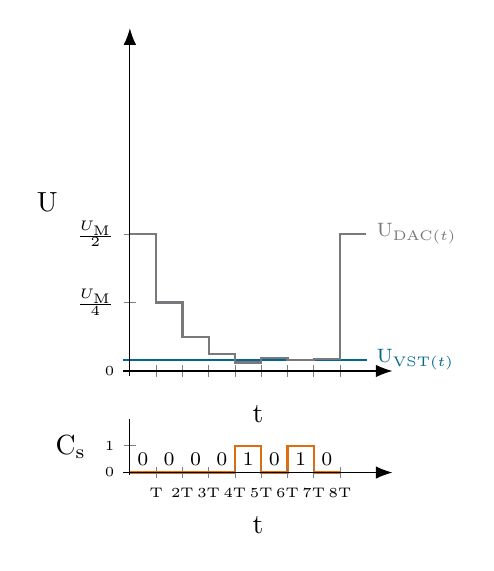
\begin{tikzpicture} [
	helper line/.style = {draw=black, ultra thin, densely dashed, mark=none},
	dim line/.style = {ultra thin, -latex, color=black},
	dim seg/.style = {ultra thin, color=black},
	digital/.style = {black, rotate=90, font=\scriptsize},
	digit/.style = {black, font=\scriptsize},
]

\definecolor{themeBlue}{RGB}{1, 103, 143}
\definecolor{themeOrange}{RGB}{221, 109, 16}
\definecolor{themeTeal}{RGB}{18, 54, 69}
\definecolor{themeGrey}{RGB}{120, 121, 124}

\begin{scope}[]
\begin{axis}[
	no markers,
    enlargelimits=false, clip=false, axis on top,
    axis lines*=middle,
    axis line style={->, -{Latex[scale=1.25]}},
    tick align=center,
    y post scale=1,
    hide obscured y ticks=false,
    %xtick=\empty, %ytick=\empty,
    xtick={0, 1, 2, 3, 4, 5, 6, 7, 8},
    xticklabels={},
    ytick={0, 2, 4},
    yticklabels={$0$, $ \frac{U_\text{M}}{4} $, $ \frac{U_\text{M}}{2} $},
	width=5cm,
	height=6cm,
	legend style={draw=none},
    jump mark left,
    ymin=-.15,ymax=10,
    xmin=-.25, xmax=10,
    xlabel={$ \text{t} $},
  	ylabel={$ \text{U} $},
	ylabel style={rotate=-90},
    every axis plot/.style={thick},
    every tick label/.append style={font=\tiny},
    discontinuous,
    table/create on use/cumulative distribution/.style={
        create col/expr={\pgfmathaccuma + \thisrow{shift}}   
    }
]
\addplot [themeBlue, smooth] coordinates {(-0.25, .33) (9, .33)} node [above, anchor=west, font=\scriptsize] {$ \text{U}_{\text{VST} (t) } $};

\addplot [themeGrey] table [y=cumulative distribution] {
x shift
0 4
1 -2
2 -1
3 -.5
4 -.25
5 .125
6 -.0625
7 .03125
8 3.655
9 0
} node [above, anchor=west, font=\scriptsize] {$ \text{U}_{\text{DAC} (t) } $};
;

\end{axis}
\end{scope}

\begin{scope}[yshift=-1.25cm]
\begin{axis}[
	no markers,
    enlargelimits=false, clip=false, axis on top,
    axis lines*=middle,
    tick align=center,
    hide obscured y ticks=false,
    x axis line style={->, -{Latex[scale=1.25]}},
    y post scale=0.5,
    %xtick=\empty, %ytick=\empty,
    xtick={0, 1, 2, 3, 4, 5, 6, 7, 8},
    xticklabels={0, T, 2T, 3T, 4T, 5T, 6T, 7T, 8T,},
    ytick={0, 2},
    yticklabels={$ 0 $, $ 1 $},
	width=5cm,
	height=3cm,
	legend style={draw=none},
    jump mark left,
    ymin=-.15,ymax=4,
    xmin=-.25, xmax=10,
    xlabel={$ \text{t} $},
  	ylabel={$ \text{C}_\text{s} $},
	ylabel style={rotate=-90},
    every axis plot/.style={thick},
    every tick label/.append style={font=\tiny},
    discontinuous,
    table/create on use/cumulative distribution/.style={
        create col/expr={\pgfmathaccuma + \thisrow{shift}}   
    }
]

\addplot [themeOrange] table [y=cumulative distribution] {
x shift
0 0
1 0
2 0
3 0
4 2
5 -2
6 2
7 -2
8 0
};

\addplot coordinates {(0.5, 1)} node [digit] {$ \text{0} $};
\addplot coordinates {(1.5, 1)} node [digit] {$ \text{0} $};
\addplot coordinates {(2.5, 1)} node [digit] {$ \text{0} $};
\addplot coordinates {(3.5, 1)} node [digit] {$ \text{0} $};
\addplot coordinates {(4.5, 1)} node [digit] {$ \text{1} $};
\addplot coordinates {(5.5, 1)} node [digit] {$ \text{0} $};
\addplot coordinates {(6.5, 1)} node [digit] {$ \text{1} $};
\addplot coordinates {(7.5, 1)} node [digit] {$ \text{0} $};

\end{axis}
\end{scope}

\end{tikzpicture}
\par}
\end{document}